\section{Autoregressive Moving Average Model}
\label{sec:ARMA}
The Autoregressive Moving Average Model (ARMA) is obtained by merging the AR and MA models. \\
Formally, the ARMA model of order $(p, q)$ is represented as follows:
\begin{equation}
    \label{eq:ARMA}
    y_{t} = \mu_{0} + \sum^{p}_{i=1}\alpha_{i} y_{t-i} + \sum^{q}_{j=1}\theta_{j} \epsilon_{t-j} + \epsilon_t 
\end{equation}
where $p$ is the number of past values considered in the AR part, $q$ is the number of past errors considered in the MA part, $\mu_{0}$ is a constant, $\alpha_{i}$ and $\theta_{j}$ are the model parameters, $y_{t-1}, y_{t-2}, ..., y_{t-p}$ are the past values, and $\epsilon_{t}, \epsilon_{t-1}, ..., \epsilon_{t-q}$ are the error terms. \\
For our analysis, we decided to implement only the ARMA(1,1) model.
\subsection*{ARMA(1,1)}
The ARMA(1,1) model is defined as:
\begin{equation}
    \label{eq:ARMA1,1}
    y_{t} = \mu_{0} + \alpha y_{t-1} + \theta \epsilon_{t-1} + \epsilon_t
\end{equation}
In our case study, we assume that $\epsilon_t$ are independent and identically distributed variables from a normal distribution with mean $0$ and variance $\sigma^2$, i.e., $\epsilon_t \stackrel{iid}{\sim} \mathcal{N}(0,\sigma^2)$, leading to the following likelihood:
\begin{equation}
    \label{eq:ARMA1,1_likelihood}
    y_{t}|\mu_{0},\alpha,\theta,\sigma^2,y_{t-1},\epsilon_{t-1} \sim \mathcal{N}(\mu_{0} + \alpha y_{t-1} + \theta \epsilon_{t-1}, \sigma^2)
\end{equation}
For the priors, we chose:
\begin{equation}
    \label{eq:ARMA1,1_priors}
    \begin{split}
        \mu_0 \sim \mathcal{N}(0.0, 10000) \\
        \tau = 1 / \sigma^2 \sim \mathcal{G}(2, 0.1) \\
        \alpha \sim \mathcal{U}(-1.0, 1.0) \\
        \theta \sim \mathcal{U}(-1.0, 1.0)
    \end{split}
\end{equation}
We selected uninformative priors for all the parameters: $\mu_{0}$, $\sigma^2$, $\alpha$, and $\theta$. \\
Running the JAGS code to implement the ARMA(1,1) model for GDP and CPIAUCSL, we obtained the posterior distributions shown in Figure \ref{fig:ARMA1,1_posteriors}, with the corresponding means and 95\% credible intervals reported in Table \ref{tab:ARMA1,1_posteriors}.
\begin{figure}[H]
    \centering
    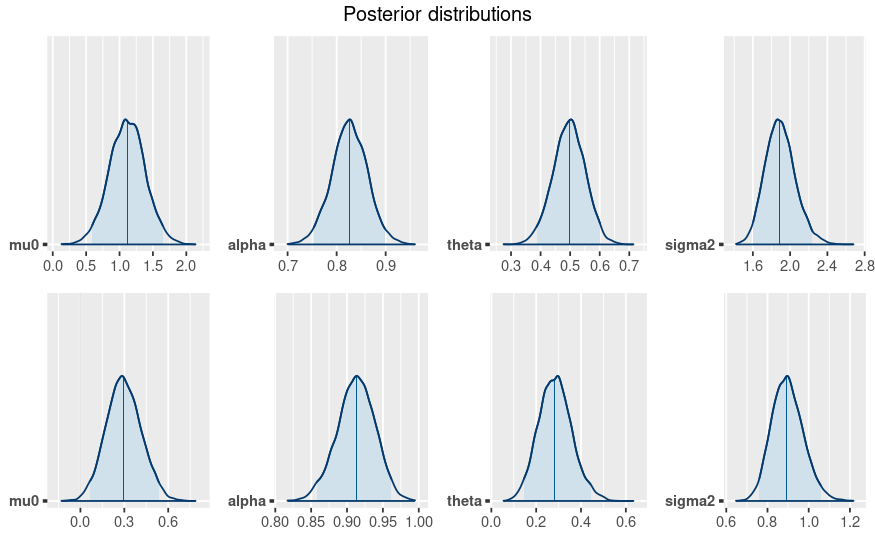
\includegraphics[width=0.8\textwidth]{images/4-ARMA/posteriors.png}
    \caption{Posterior distributions of the parameters for the ARMA(1,1) models. The top line corresponds to the model used for GDP, while the bottom line corresponds to the model used for CPIAUCSL.}
    \label{fig:ARMA1,1_posteriors}
\end{figure}
\begin{table}[H]
    \centering
    \begin{tabular}{|c|c|c|c|}
        \hline
        \textbf{Model target variable } & \textbf{Parameter } & \textbf{Posterior Mean } & \textbf{95\% Credible Interval } \\
        \hline
        GDP      & $\mu_0$    & 1.1207710 & (0.59421700, 1.6538357) \\
        GDP      & $\alpha$   & 0.8254802 & (0.75268077, 0.8966752) \\
        GDP      & $\theta$   & 0.4952213 & (0.38504175, 0.6024967) \\
        GDP      & $\sigma^2$ & 1.8977382 & (1.60426034, 2.2438487) \\
        CPIAUCSL & $\mu_0$    & 0.2941814 & (0.07023124, 0.5314746) \\
        CPIAUCSL & $\alpha$   & 0.9127231 & (0.86025773, 0.9612327) \\
        CPIAUCSL & $\theta$   & 0.2846962 & (0.14830563, 0.4392942) \\
        CPIAUCSL & $\sigma^2$ & 0.8976673 & (0.75858882, 1.0607612) \\
        \hline
    \end{tabular}
    \caption{Posterior means and 95\% credible intervals for the parameters of the ARMA(1,1) models.}
    \label{tab:ARMA1,1_posteriors}
\end{table}
Plotting the in-sample and out-of-sample predictions with 95\% credible intervals and comparing them with the actual data, we obtained the results shown in Figures \ref{fig:ARMA1,1_gdp_prediction} and \ref{fig:ARMA1,1_infl_prediction}. \\
The out-of-sample predictions for GDP and CPIAUCSL effectively capture the initial data trends. Nevertheless, the ARMA(1,1) model fails to anticipate the significant impact of the COVID-19 pandemic, which is completely understandable.
\begin{figure}[H]
    \centering
    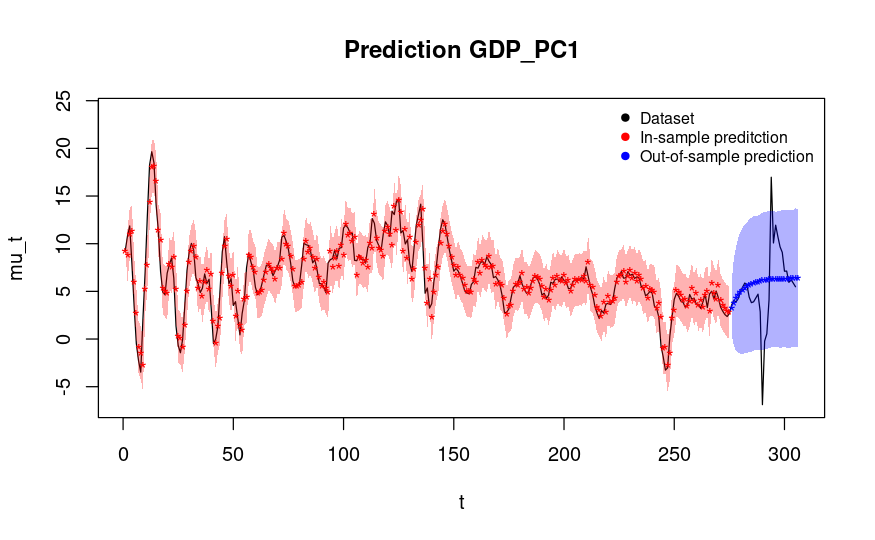
\includegraphics[width=0.75\textwidth]{images/4-ARMA/gdp_prediction.png}
    \caption{In-sample and out-of-sample predictions for the GDP using the ARMA(1,1) model.}
    \label{fig:ARMA1,1_gdp_prediction}
\end{figure}
\begin{figure}[H]
    \centering
    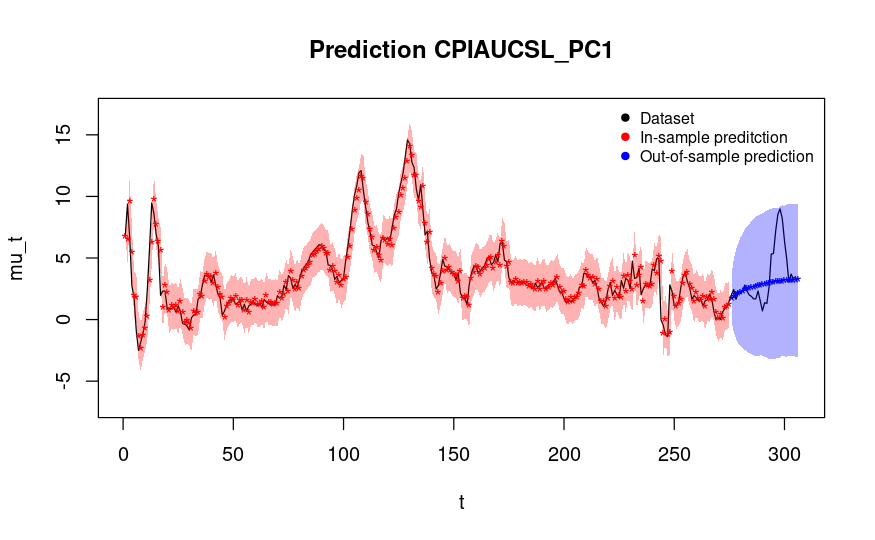
\includegraphics[width=0.75\textwidth]{images/4-ARMA/infl_prediction.png}
    \caption{In-sample and out-of-sample predictions for the CPIAUCSL using the ARMA(1,1) model.}
    \label{fig:ARMA1,1_infl_prediction}
\end{figure}
Finally, examining the trace plots and autocorrelation plots, we found no significant issues, and comparing our model with the one obtained using the ARIMA function, we observed that the two models have similar results. Results are provided in the Appendix.